\documentclass[manuscript,screen,nonacm]{acmart}
\setcopyright{none}
\settopmatter{printacmref=false,printccs=false}
\acmDOI{}
\acmISBN{}
\usepackage{longtable,booktabs,array,calc,xurl,fvextra,tikz}
\usetikzlibrary{positioning}
\DefineVerbatimEnvironment{verbatim}{Verbatim}{breaklines=true,fontsize=\small}
\providecommand{\tightlist}{\setlength{\itemsep}{0pt}\setlength{\parskip}{0pt}}
\usepackage{graphicx,float}

% Permit figures to share pages with surrounding explanatory text.
\renewcommand{\topfraction}{0.92}
\renewcommand{\bottomfraction}{0.85}
\renewcommand{\textfraction}{0.06}
\renewcommand{\floatpagefraction}{0.80}
\setcounter{topnumber}{3}
\setcounter{bottomnumber}{3}
\setcounter{totalnumber}{5}
\setlength{\textfloatsep}{12pt plus 2pt minus 3pt}
\setlength{\intextsep}{12pt plus 2pt minus 3pt}
\raggedbottom

\geometry{left=1in,right=1in,top=0.75in,bottom=0.65in,includeheadfoot}
\begin{document}
\title{Emotional Atlas: Emotional Geometry, Textual Evolution, and Shape-Guided Revision}
\author{William Taggart}
\affiliation{\department{Modern and Classical Languages and Literatures}
\institution{Virginia Tech}\city{Blacksburg}\state{Virginia}\country{USA}}
\email{wtaggart@vt.edu}
\subtitle{Technical report on version 0.9.10; November 13, 2026}
\begin{abstract}
Emotional Atlas is a desktop environment for examining emotional
movement in literary texts and dream reports. It combines large language
model (LLM) inference with locally validated textual evidence, a
three-coordinate emotional representation, interactive visualization,
geometric construction, and text-order evolution. A separate
multilingual idiom workflow proposes direct expressions, transformed
expressions, and tentative imagery echoes. An emotional shape-transfer
workspace uses the trajectory of a source analysis to guide revision of
another text. The system supports conservative editing and a more
permissive transformation policy, reports its decisions, and preserves
resumable checkpoints. This report describes the implemented algorithms,
data flow, operational constraints, and verification of version 0.9.10.
The scores and interpretations are model judgments, not established
psychometric measurements; software verification does not establish
interpretive accuracy or transfer efficacy.
\end{abstract}
\keywords{emotional geometry, text analysis, shape transfer, multilingual idioms, visualization}
\maketitle
\section{Scope and design}\label{scope-and-design}

The application supports exploratory reading and computational
experimentation. Its central unit is a text segment: ordinarily a
paragraph, optionally a line, or a sentence when granular analysis is
enabled. The interface preserves a distinction between source text,
inferred emotional descriptions, derived coordinates, and geometric
representations. Changing a surface or viewing mode does not change the
underlying scores.

The main window contains text input, provider controls, the primary
scatter plot, results, and evidence inspection. Expanded plots,
solid/evolving objects, and shape transfer use separate windows. Dark
mode is the startup default; a Light option changes interface
backgrounds and text across open and newly created windows. Valence
colors, yellow idiom markers, and user-selected surface colors remain
distinct from interface appearance.

This report describes implemented functionality. It does not claim that
emotional meaning has a unique geometric form, that a dream image has a
determinate symbolic meaning, or that generated revisions preserve facts
in flexible mode.


\subsection{Research context}

Dimensional models provide a research context for emotional coordinates. Russell's circumplex organizes affect around valence and arousal \cite{russell}, while Bradley and Lang's Self-Assessment Manikin includes pleasure, arousal, and dominance in human ratings \cite{sam}. Word-level affective norms from Warriner and colleagues \cite{warriner} and the NRC VAD lexicon \cite{vad} provide empirical reference points. These resources concern annotated stimuli and populations; they do not validate an LLM's scores for a paragraph or a dream. GoEmotions offers a complementary categorical annotation scheme \cite{goemotions}, illustrating why categories and continuous dimensions should not be treated as interchangeable measurements.

Reagan and colleagues analyze emotional trajectories in a literary corpus \cite{arcs}. Their study motivates examining change over text order, but it does not establish universal narrative templates or validate the present segmentation and scoring procedure. PCA summarizes variation through a linear projection \cite{pca}; the retained variance and shared projection basis therefore matter when comparing displayed trajectories. Alpha-shape research formalizes families of boundaries constructed from point sets \cite{alphashapes}. It offers a geometric comparison for the app's solid-object views, not evidence that a rendered boundary measures emotional meaning or that every surface option implements an alpha shape.

Text style-transfer research separates attribute control from content preservation and fluency \cite{style}. Emotional shape transfer similarly needs separate checks of coordinate agreement, readability, and semantic change, especially when flexible rewriting is enabled. Multilingual idiomaticity benchmarks evaluate expressions in context \cite{idioms}. Inferring an idiom from dream imagery extends beyond that benchmark setting: an image resembling a literal expression is a hypothesis for reader review, not proof of the dreamer's intention.

\section{Architecture and execution}\label{architecture-and-execution}

The application is written in Python with Tk/ttk. Network inference runs
in worker threads, with queued events delivered to the GUI. Geometry and
export operations also use background work where implemented. Local
plotting, playback, PCA, and saved-result inspection do not require new
model requests.

\begin{figure}[!htb]
\centering
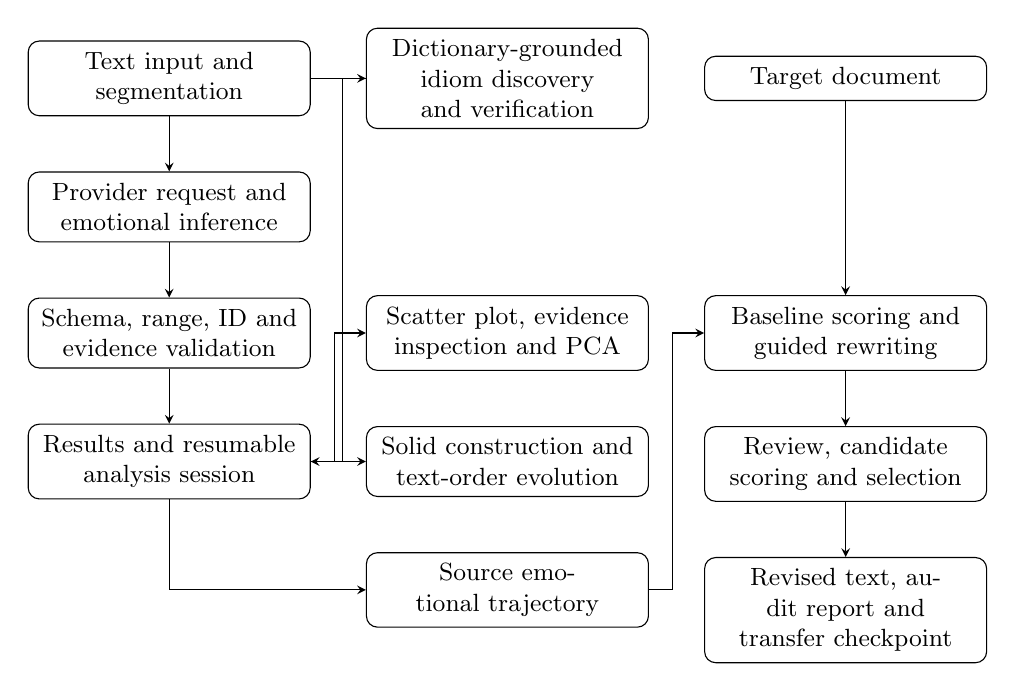
\begin{tikzpicture}[node distance=7mm and 7mm,
 box/.style={draw,rounded corners,align=center,font=\small,text width=33mm,inner sep=4pt},
 arr/.style={->,>=stealth}]
\node[box] (a) {Text input and segmentation};
\node[box,below=of a] (b) {Provider request and emotional inference};
\node[box,below=of b] (c) {Schema, range, ID and evidence validation};
\node[box,below=of c] (d) {Results and resumable analysis session};
\node[box,right=of a] (l) {Dictionary-grounded idiom discovery and verification};
\node[box,right=of c] (e) {Scatter plot, evidence inspection and PCA};
\node[box,below=of e] (f) {Solid construction and text-order evolution};
\node[box,below=of f] (g) {Source emotional trajectory};
\node[box,right=of l] (h) {Target document};
\node[box,right=of e] (i) {Baseline scoring and guided rewriting};
\node[box,below=of i] (j) {Review, candidate scoring and selection};
\node[box,below=of j] (k) {Revised text, audit report and transfer checkpoint};
\draw[arr] (a)--(b);\draw[arr] (b)--(c);\draw[arr] (c)--(d);
\draw[arr] (a)--(l);\draw[arr] (l.west)--++(-3mm,0)|-(d.east);
\draw[arr] (d.east)--++(3mm,0)|-(e.west);\draw[arr] (d)--(f);
\draw[arr] (d.south)|-(g.west);\draw[arr] (g.east)--++(3mm,0)|-(i.west);
\draw[arr] (h)--(i);\draw[arr] (i)--(j);\draw[arr] (j)--(k);
\end{tikzpicture}
\caption{Emotional Atlas analysis, visualization, idiom, and shape-transfer workflows.}
\Description{Text passes through inference and validation to resumable results. Results feed plots, solid evolution and a source trajectory. Idiom verification feeds results. The source trajectory and target text feed rewriting, review and export.}
\end{figure}

{ % do not increment counter
\begin{longtable}[]{@{}
  >{\raggedright\arraybackslash}p{(\linewidth - 2\tabcolsep) * \real{0.5000}}
  >{\raggedright\arraybackslash}p{(\linewidth - 2\tabcolsep) * \real{0.5000}}@{}}
\toprule\noalign{}
\begin{minipage}[b]{\linewidth}\raggedright
Component
\end{minipage} & \begin{minipage}[b]{\linewidth}\raggedright
Responsibility
\end{minipage} \\
\midrule\noalign{}
\endhead
\bottomrule\noalign{}
\endlastfoot
\nolinkurl{app.py} & Main interface, canvas plotting, source/session
controls and orchestration \\
\nolinkurl{analysis.py} & Provider adapters, inference prompt, validation,
evidence repair and session serialization \\
\nolinkurl{segmentation.py} & Local sentence-boundary heuristics \\
\nolinkurl{pca.py}, \nolinkurl{playback.py} & Standardized PCA and text-order
playback \\
\nolinkurl{idioms.py}, \nolinkurl{datasets/} & Idiom retrieval, verification
and dictionary provenance \\
\nolinkurl{geometry.py}, \nolinkurl{object_view.py} & Solid construction,
subdivision, rendering and object export \\
\nolinkurl{evolution_export.py} & Bounded, cancellable evolution export \\
\nolinkurl{shape_transfer.py}, \nolinkurl{transfer_view.py} & Trajectory
alignment, rewriting, selection and transfer interface \\
\nolinkurl{transfer_session.py}, \nolinkurl{session_identity.py} & Transfer
checkpoints and distinct timestamped session identities \\
\nolinkurl{appearance.py} & Light/dark interface palette \\
\nolinkurl{smoke.py}, \nolinkurl{test_*.py} & Offline native checks and
automated regression tests \\
\end{longtable}
}

The configured OpenAI adapter uses the Responses API and model
identifier \nolinkurl{gpt-6-luna}. VT ARC uses a Chat
Completions-compatible endpoint, defaults to \nolinkurl{gpt-oss-120b}, and
permits a user-specified model identifier. These are software
configuration values, not guarantees of provider availability. The
application does not silently substitute another model. Transfer uses
the source analysis's provider/model to reduce one source of scoring
inconsistency.

Model judgments are checked locally against the source text before eligible segments enter the geometry. These checks establish consistency with the expected response structure and quoted evidence; they do not establish psychometric accuracy.

\section{Emotional inference and
evidence}\label{emotional-inference-and-evidence}

\subsection{Representation}\label{representation}

For segment i, the model returns intensity \(I_i\) in {[}0,1{]}, valence
\(V_i\) in {[}-1,1{]}, and direction \(D_i\) in {[}-1,1{]} or an unknown
value. Intensity denotes strength of feeling rather than physical
activity or arousal. Valence runs from unpleasant to pleasant. Direction
runs from inward/self-focused to directed toward another person, object,
or the world.

The response also contains tone, an ordinal uncertainty judgment, a
summary, and up to five emotional experiences. Each experience
identifies an experiencer, target where supported, emotional scores,
explanations, and evidence. Opposing feelings can remain separate even
when net valence is near zero. Low/medium/high uncertainty is not a
calibrated probability.

The prompt asks the model to distinguish expressed emotion from negated,
hypothetical, quoted, or merely mentioned emotion and to consider
metaphor, irony, and speaker changes. These are instructions to the
model, not demonstrated guarantees.

\subsection{Validation and recovery}\label{validation-and-recovery}

Local validation checks response structure, IDs, numeric ranges,
directional consistency, and evidence correspondence. Evidence must
resolve to source wording; limited normalization accommodates formatting
differences without introducing fuzzy semantic matching. Signal words
must be supported by the quoted evidence. Nearby context is supplied for
interpretation but is not a valid substitute for evidence in the target
segment.

Ordinary analysis batches contain up to six units under an
18,000-character target-text budget. An individual oversized unit can
exceed that batching budget, subject to the analysis unit limit.
Neighboring context is bounded to 1,200 characters on each side. The
system therefore does not maintain complete book-length context.

Valid results are retained when a neighboring segment fails. Failed
evidence may be repaired through source-word selection. Passage-specific
response or repair failures are marked for review and processing
continues. Provider, account, transport, or certificate failures stop
the run rather than being misclassified as textual failures. Stop is
cooperative; an active network request can take up to its 150-second
timeout to return. No fallback emotional scores are fabricated.

\subsection{Segmentation}\label{segmentation}

Sentence analysis is opt-in. The local heuristic recognizes common
English, Arabic, and Chinese terminal punctuation, selected
abbreviations, decimal patterns, and closing punctuation. It is not a
trained multilingual sentence parser. Dialogue, unusual abbreviations,
poetry, and punctuation-free text can be segmented imperfectly. Changing
analysis granularity starts a separate analysis; saved metadata
identifies the segmentation mode even where legacy fields retain names
such as \nolinkurl{paragraphs}.


\section{Emotional geometry and PCA}\label{emotional-geometry-and-pca}



The primary plot places each eligible text segment at a point with three coordinates. The horizontal x coordinate is valence, ranging from unpleasant (-1) to pleasant (+1). The y coordinate is emotional direction, ranging from inward or self-focused (-1) to directed toward another person, object, or the world (+1). The z coordinate represents emotional intensity: the original intensity score is doubled and then reduced by one, so an intensity of 0 appears at -1, an intensity of 0.5 at 0, and an intensity of 1 at +1.

This conversion puts all three display axes on the same numeric range without changing the ordering of intensity scores. Equal axis ranges are a modeling convention, not an empirically established equality of emotional distances. Point color normally represents valence; an idiom annotation can instead mark a point in yellow.

\begin{figure}[!htb]
\centering
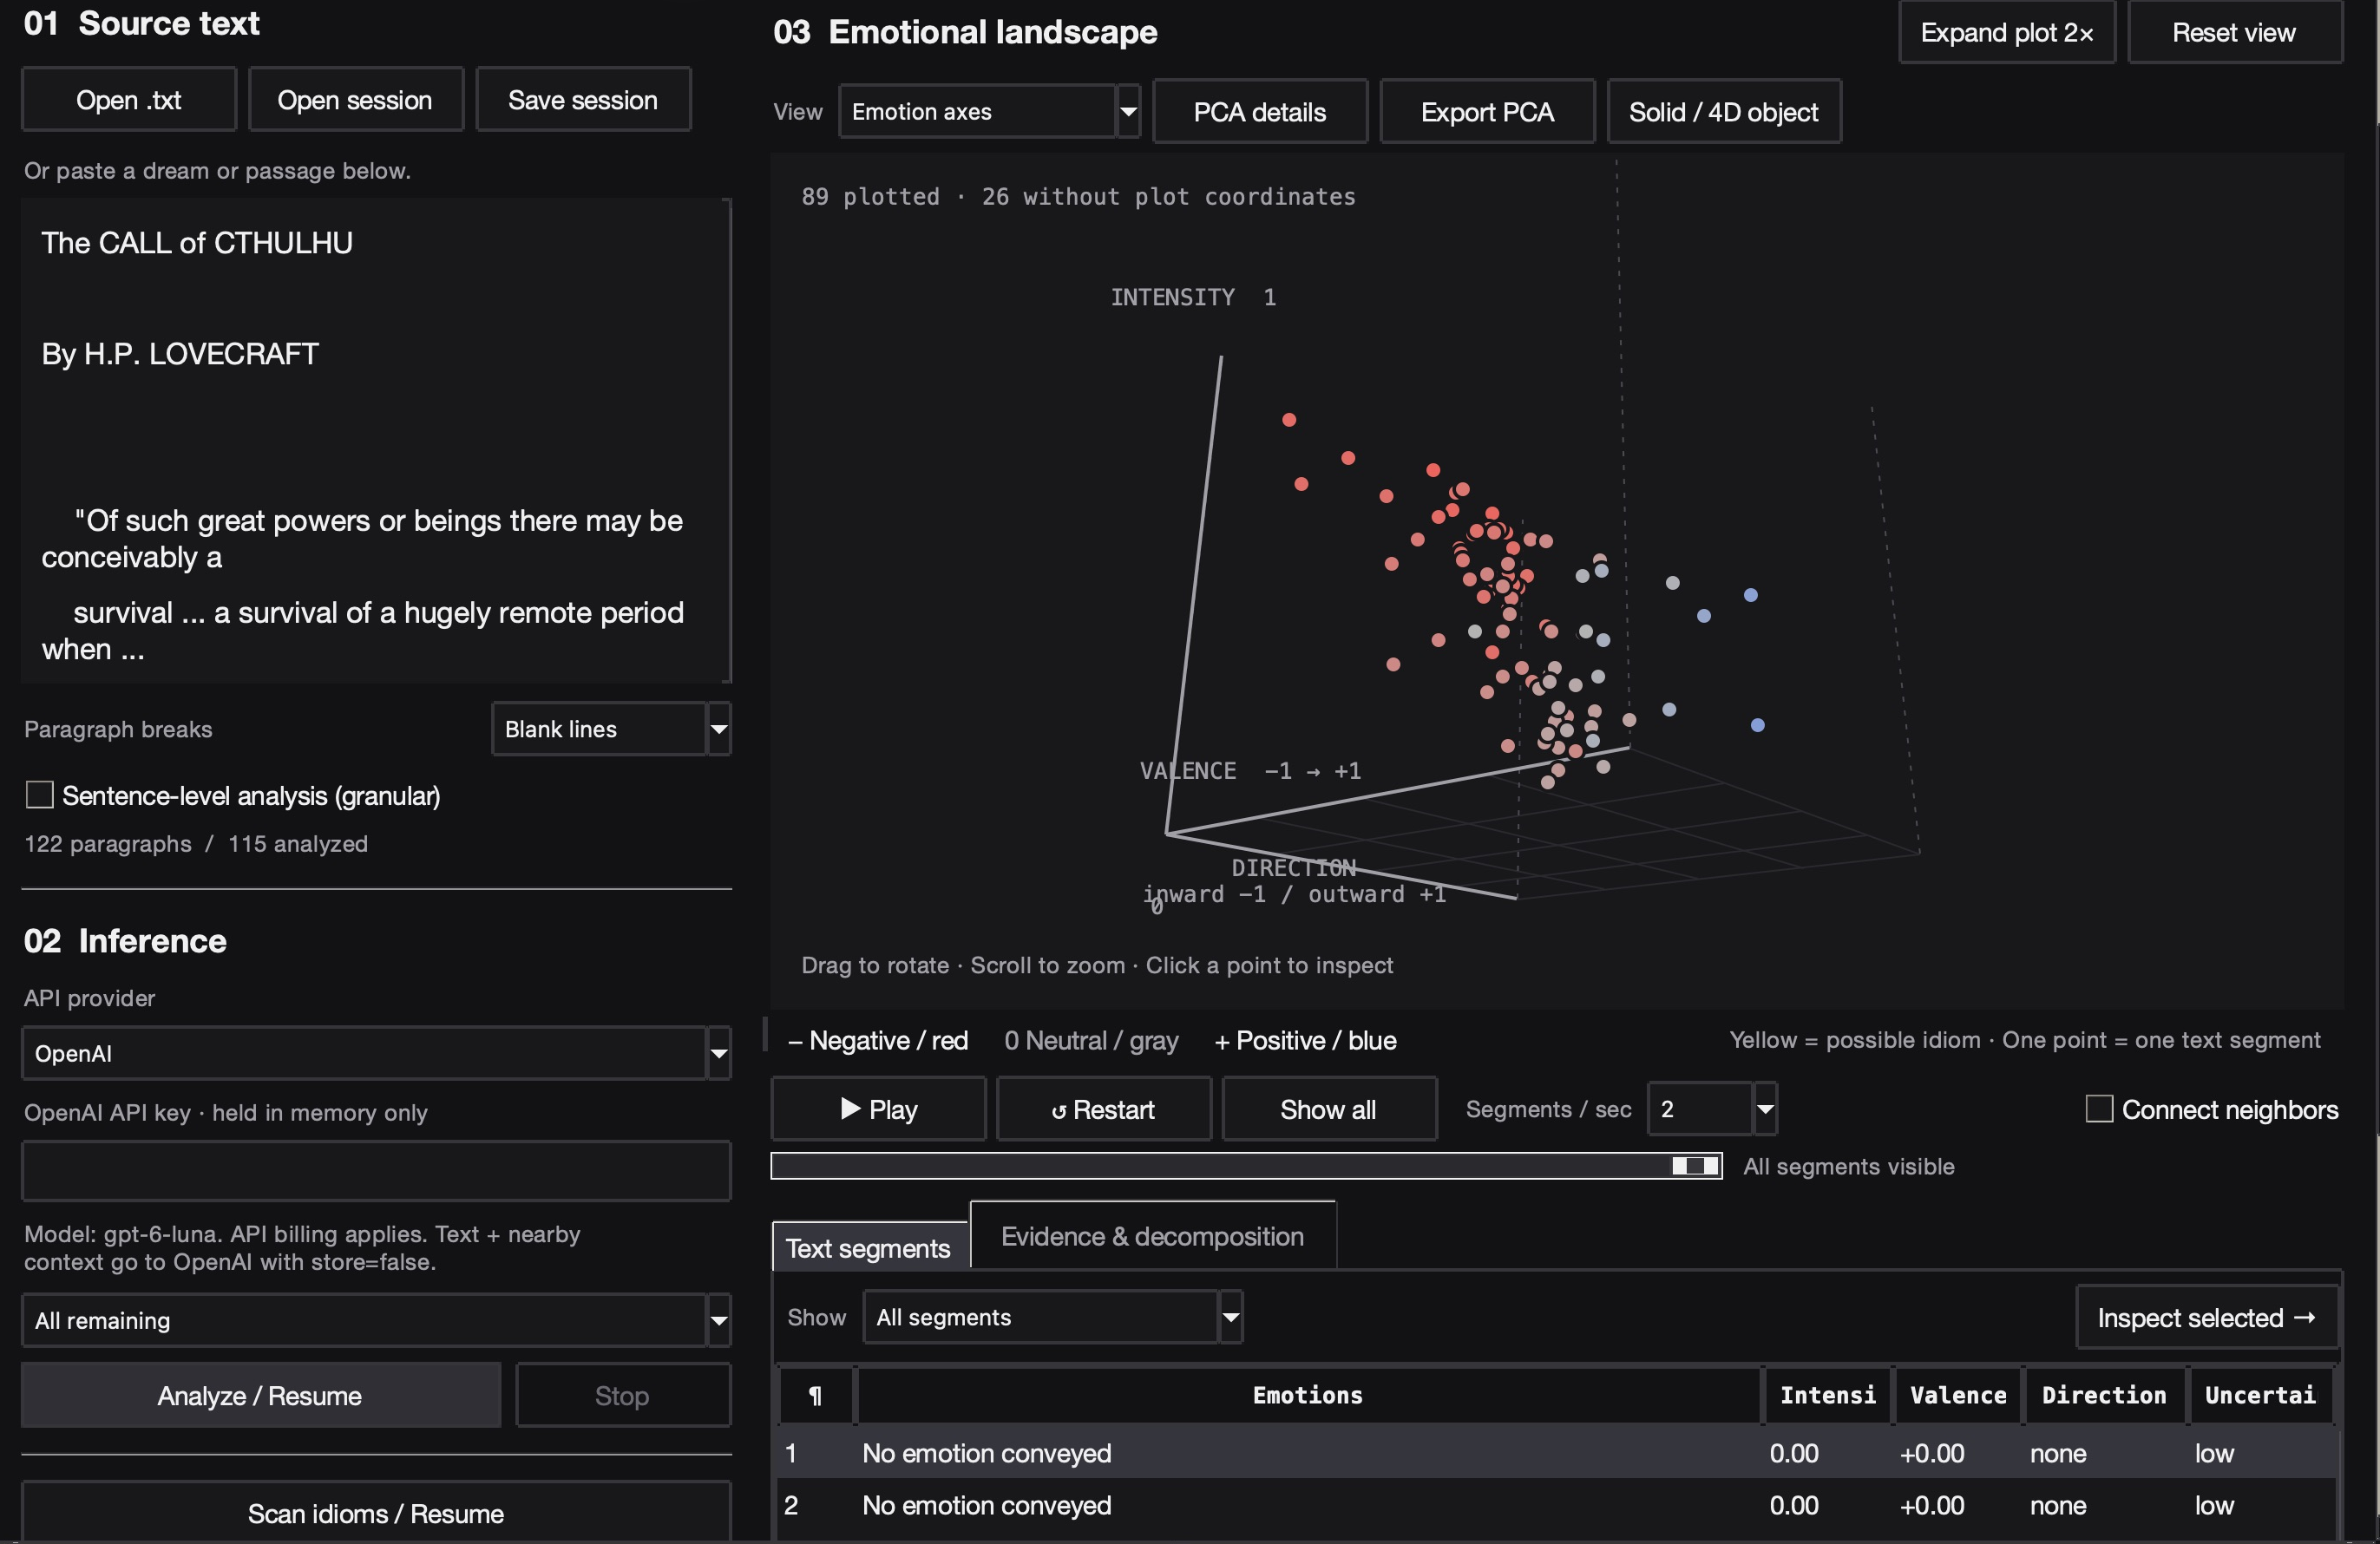
\includegraphics[width=.88\linewidth,height=0.58\textheight,keepaspectratio]{figures/screenshot-01.png}
\caption{Saved analysis of The Call of Cthulhu, with 89 plotted paragraphs and 26 analyzed paragraphs lacking plot coordinates. Point colors encode valence.}
\Description{Saved analysis of The Call of Cthulhu, with 89 plotted paragraphs and 26 analyzed paragraphs lacking plot coordinates. Point colors encode valence.}
\label{fig:app-screen-1}
\end{figure}

Unknown direction is not replaced with zero. Such segments remain
available in the results but lack a full 3D coordinate and are excluded
from geometry. Thus an empty original-target plot does not by itself
establish emotional neutrality: it can indicate unsupported direction.
Identical coordinates can also overlap.

PCA operates on the three existing scores, not on text embeddings. Each
nonconstant feature is centered and divided by its sample standard
deviation. A Jacobi eigendecomposition of the resulting 3-by-3
covariance matrix supplies components and explained-variance ratios.
Constant features contribute zero. At least three eligible segments and
nonzero variation are required. Retaining all three PCs preserves the
variance of these three inputs; it does not preserve every semantic
feature of the text. Component signs are conventional, and nearly equal
eigenvalues can make individual axes unstable.

The evolving-object view fits PCA once to its full snapshot and retains
the same basis and display scale across frames. This avoids apparent
motion caused solely by refitting the coordinate system at each time
step.

\section{Solid objects, curved surfaces and
evolution}\label{solid-objects-curved-surfaces-and-evolution}


\begin{figure}[!htb]
\centering
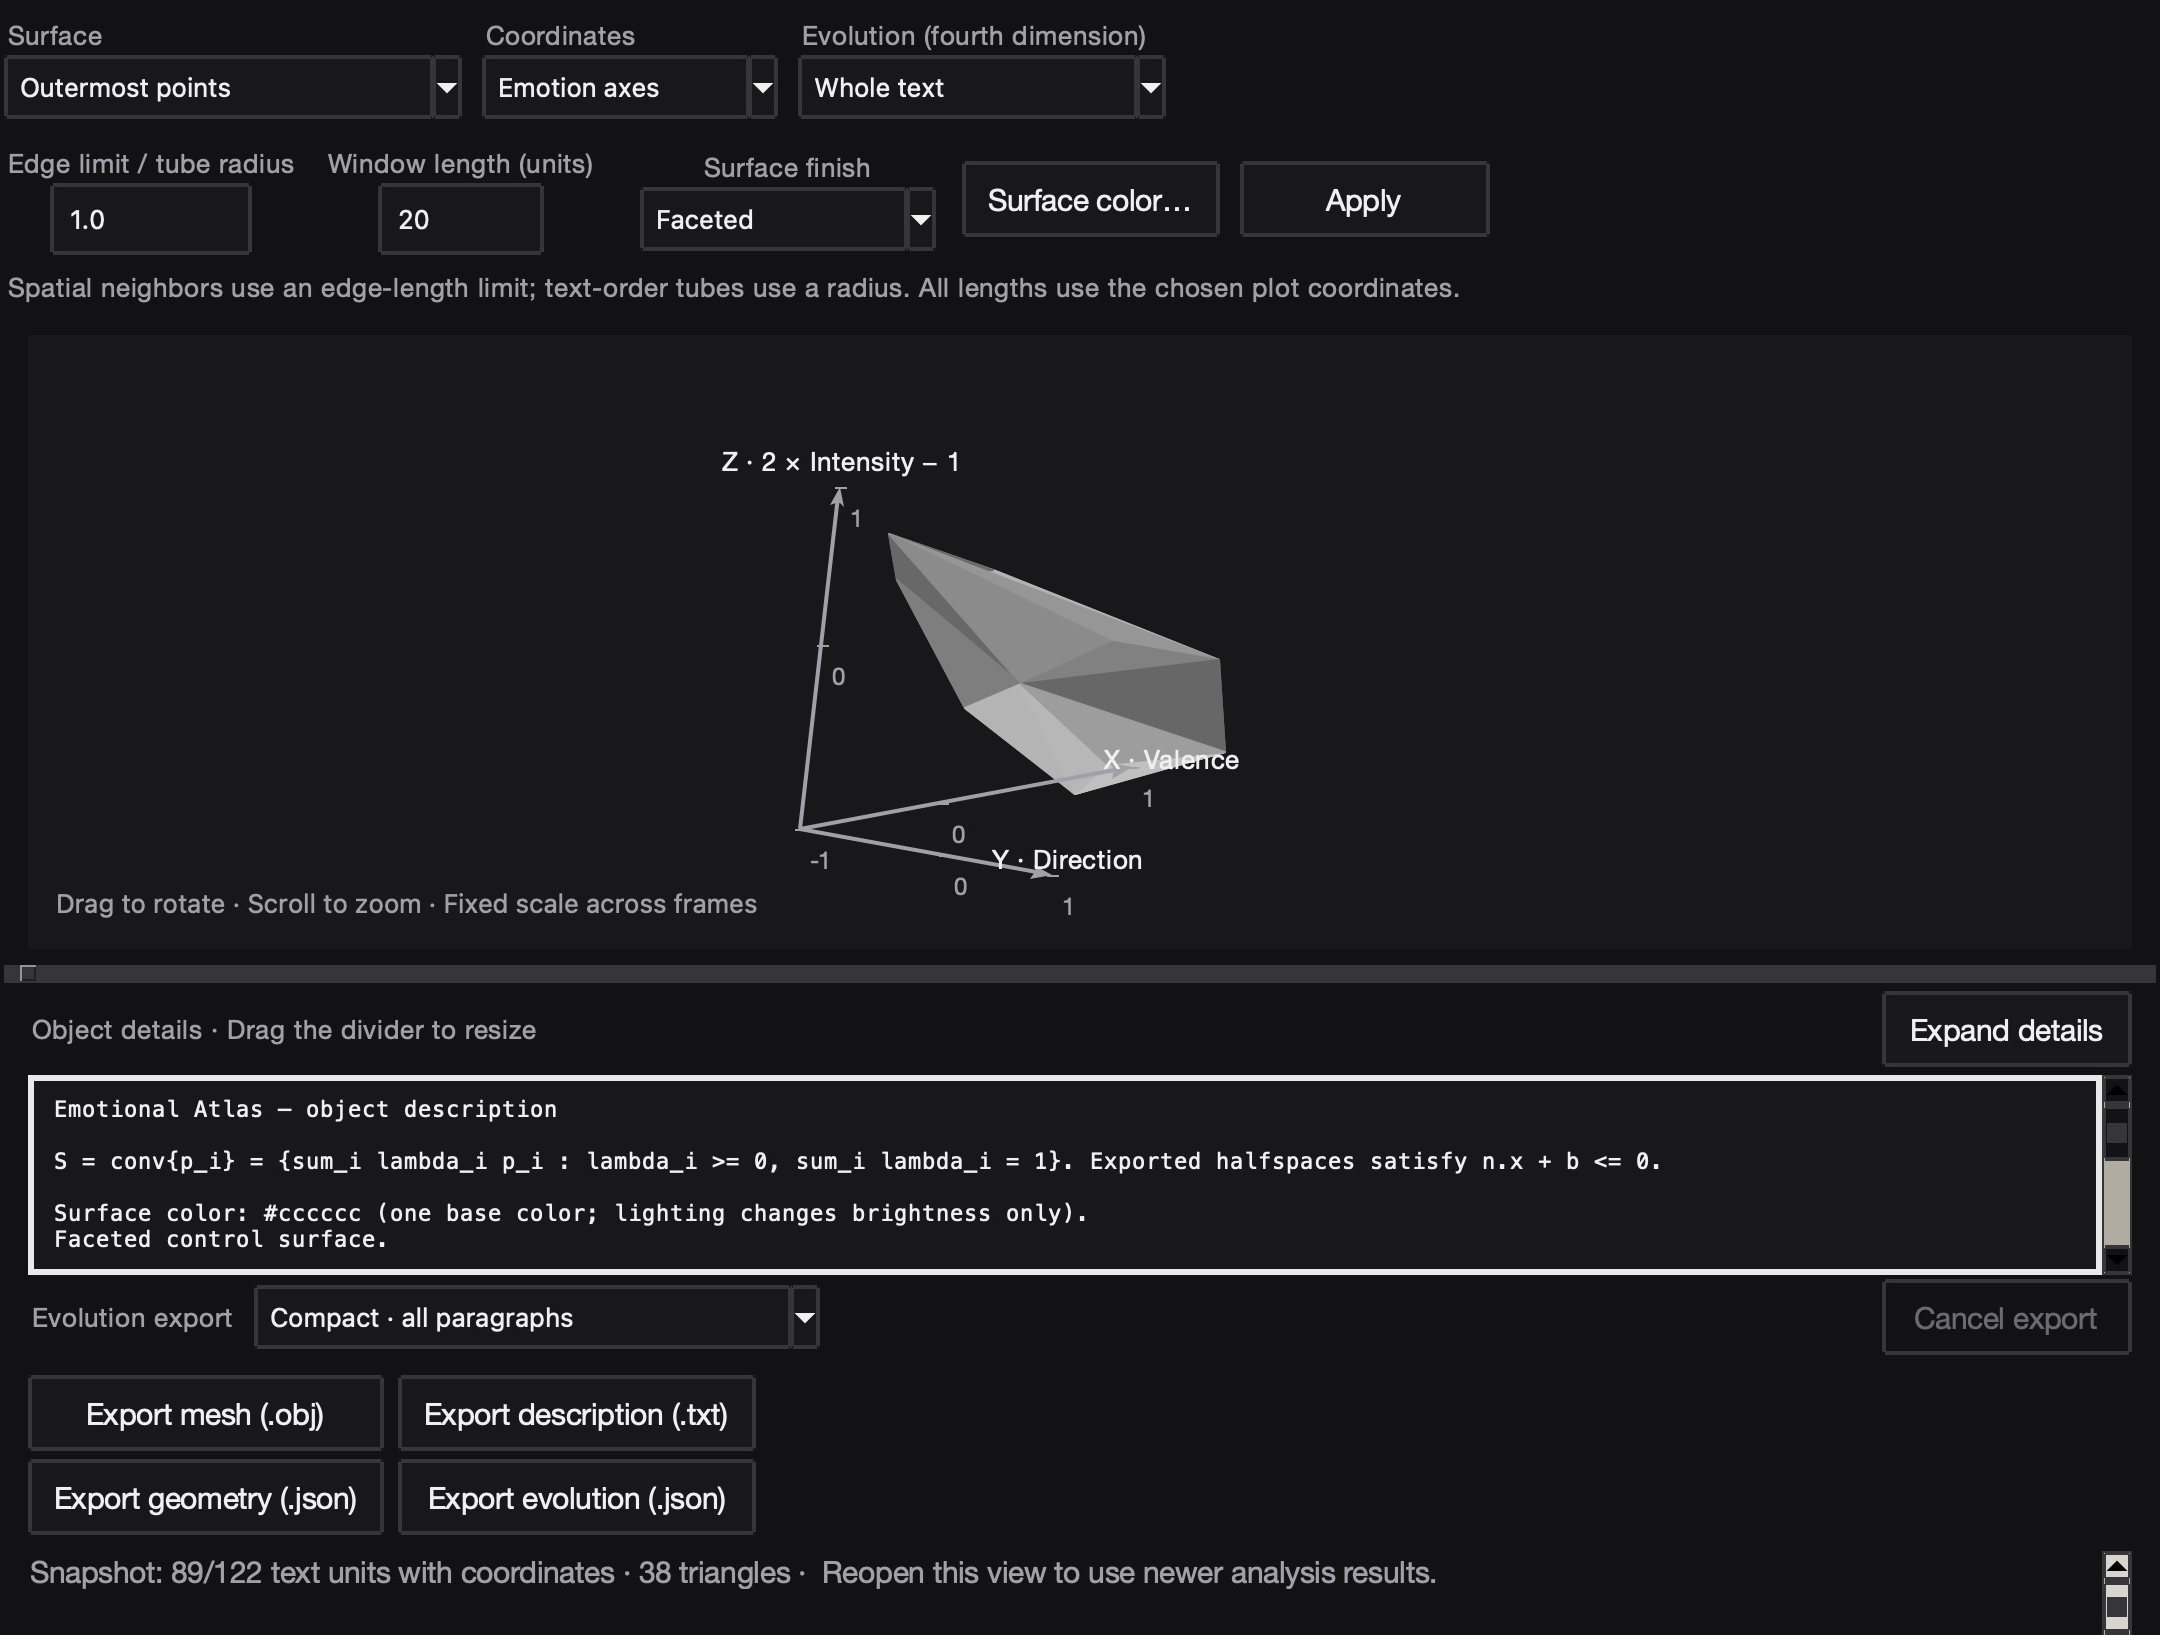
\includegraphics[width=.88\linewidth,height=0.58\textheight,keepaspectratio]{figures/screenshot-02.png}
\caption{Solid-object window showing the outermost-point surface, labeled emotional axes, mathematical description, and export controls for the saved analysis.}
\Description{Solid-object window showing the outermost-point surface, labeled emotional axes, mathematical description, and export controls for the saved analysis.}
\label{fig:app-screen-2}
\end{figure}
Three constructions are implemented:

\begin{enumerate}
\def\labelenumi{\arabic{enumi}.}
\tightlist
\item
  \textbf{Outermost points:} the convex hull of unique eligible points.
  It encloses the sample but fills gaps and concavities.
\item
  \textbf{Spatial neighbors:} a 3D Delaunay tetrahedralization filtered
  by a maximum-edge-length threshold. Exterior faces of retained
  tetrahedra form the surface. This is a specific thresholded
  tetrahedral construction, not a general claim to recover the text's
  intrinsic topology. It may produce disconnected components, cavities
  or nonmanifold contacts.
\item
  \textbf{Text-order tube:} polygonal rings swept along consecutive
  emotional positions, with caps on connected runs. Missing coordinates
  break the path. Thickness is user-controlled, and crossings or tight
  bends can self-intersect; tube volume is not claimed.
\end{enumerate}

Coplanar or collinear samples do not define a full-dimensional hull. The
interface explains such cases instead of inventing thickness. NumPy and
SciPy provide numerical operations and hull/tetrahedral computations.

One to three Loop subdivision steps create tessellated approximations to
curved surfaces from suitable closed manifold control meshes. Each step
replaces a triangle with four and updates vertices through weighted
neighbor averages. Smoothing generally rounds and shrinks a shape: a
smoothed hull need not contain every source point. Area and eligible
volume are recomputed from the resulting mesh. A single chosen surface
color is shaded to convey depth; OBJ export includes a corresponding MTL
file.

The fourth coordinate is normalized text order:

\[\tau_i=\frac{i-1}{N-1},\]

with zero used for a one-unit text. Cumulative evolution includes
eligible points through i; moving-window evolution includes positions
\(\max(1,i-w+1)\) through i. Missing coordinates still occupy timeline
positions. The displayed sequence is a family of 3D slices \(S_i\),
conceptually defining:

\[W=\bigcup_{i=1}^{N-1}S_i\times[\tau_i,\tau_{i+1}),\]

plus the final slice at the endpoint. This is text-order evolution, not
elapsed reading time or a projected 4D convex hull. Topology can change
between slices, and unmatched vertices are not interpolated.


\section{Multilingual idioms and dream
imagery}\label{multilingual-idioms-and-dream-imagery}

Idiom scanning is a separate workflow. It distinguishes possible direct
use, transformed expressions, and imagery echoes. One request proposes
canonical expressions; local retrieval grounds candidates in available
dictionary entries; a subsequent request verifies retrieved candidates
against the passage. Known dictionary IDs and source quotes are checked
locally.

The bundled inventory contains 20 English and 10 Arabic starter
expressions with project-authored glosses, plus 30,895 Chinese records
adapted from \nolinkurl{pwxcoo/chinese-xinhua}, revision
\nolinkurl{fe6d6c2e8baa82187f4c96bbe042e43f96c05666}. Its MIT license and
attribution are retained in the repository. Inventory size does not
measure detection accuracy. English/Arabic coverage is preliminary;
dialect variation and Chinese traditional/simplified normalization
remain limitations. Imported dictionaries extend coverage and must
supply IDs, language, phrase, meaning, source and license metadata.

An image such as someone taking a goat could be proposed as an echo of
``get your goat,'' but lexical overlap or an object alone is
insufficient proof. Alternative readings are presented. These
annotations are interpretive hypotheses, not explanations of a dreamer's
mental state. ChengyuBench is identified in project documentation as a
potential evaluation resource; it is not bundled or used to establish
the system's accuracy.

\begin{figure}[!htb]
\centering
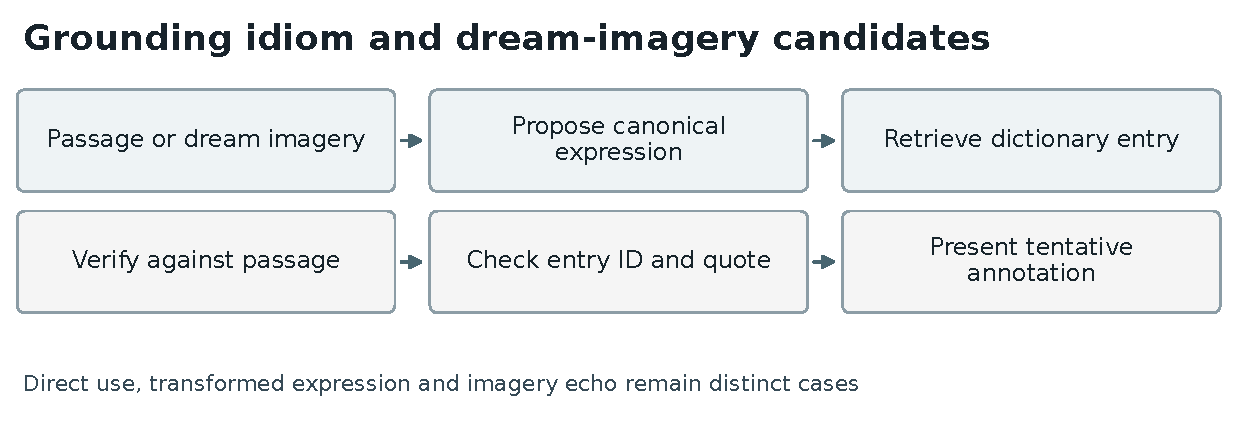
\includegraphics[width=.9\textwidth]{figures/illustration-04.pdf}
\caption{Idiom workflow. A literal image alone is not proof of an idiom; retrieved expressions and quoted evidence support hypotheses with alternative readings.}
\Description{Grounding idiom and dream-imagery candidates. Idiom workflow. A literal image alone is not proof of an idiom; retrieved expressions and quoted evidence support hypotheses with alternative readings.}
\label{fig:illustration-4}
\end{figure}

\section{Emotional shape transfer}\label{emotional-shape-transfer}

\subsection{Alignment and objective}\label{alignment-and-objective}

Transfer snapshots the source analysis directly from memory. No mesh
export is required. It uses the raw emotional trajectory, not PCA
coordinates, a convex hull, Loop-smoothed surface, or chosen surface
color.

Known source coordinates form a piecewise-linear trajectory \(p(t)\)
over normalized source-unit positions. Gaps are interpolated and
positions beyond the known range clamp to the nearest endpoint. A target
with M processing units samples \(t_j=(j-1)/(M-1)\); a one-unit target
samples \(t=0.5\). With baseline target point \(b_j\) and strength s:

\[q_j=(1-s)b_j+s\,p(t_j).\]

If the baseline lacks a supported direction, the complete baseline point
is unavailable and \(q_j\) is set to \(p(t_j)\). Candidate distance is:

\[e_j=\frac{\lVert c_j-q_j\rVert_2}{2\sqrt{3}}.\]

This normalizes distance by the cube diagonal. It is not a calibrated
measure of literary quality. Resampling trajectories does not guarantee
equal hulls, volume, or topology.

\subsection{Generation, review and
selection}\label{generation-review-and-selection}

The workflow scores the original target, generates a revision, reviews
it, scores the candidate without supplying desired coordinates to the
scorer, and finally scores the assembled result in its revised
neighboring context. One or two revision attempts can be selected. A
second attempt receives feedback from the first. The original,
requested, and revised trajectories are displayed separately.

\textbf{Flexible transformation}, the default, permits substantial
changes to imagery, perspective, emotional reactions, supporting details
and local events. The review asks whether the result remains coherent,
readable and recognizably related to the target. Meaning and numeric
changes are disclosed rather than used as automatic vetoes. Among
reasonable scored revisions actually generated, the closest is
selected---even if the original scored closer. This policy favors
transformation but cannot promise improvement or factual fidelity.

\textbf{Preserve meaning} requires a review with no semantic concerns,
unchanged numeric content under the local check, supported direction,
and a lower distance than the current best. The original or a prior
accepted candidate remains when no candidate qualifies. Neither policy
is a global optimization procedure or a guarantee of an exact emotional
match. The reviewer and scorer can share model biases; a separate API
call does not constitute independent human validation.

\subsection{Long documents, boundaries and
failures}\label{long-documents-boundaries-and-failures}

There is no fixed document-length or unit-count cap in transfer
preparation. Oversized units are divided internally into passages of at
most 3,000 characters, preferring sentence boundaries and then
whitespace. Target request batches use up to six units and a
6,000-character text budget; surrounding context and structured metadata
add to actual request size. Users load and export one document. Original
separators are retained between spans; replacement text can introduce
additional sentence or paragraph boundaries within a span. The entire
replacement is scored under its original ID. A subsequent sentence-level
reanalysis may therefore produce a different number of points.

A normal one-attempt batch uses approximately five model calls before
correction, retries or failure isolation; two attempts add another
rewrite/review/scoring cycle. Long documents can require substantial
time and API usage. Completed-response usage counters can undercount
requests whose responses were interrupted or rejected before accounting
was returned.

Passage-specific failures trigger bounded batch isolation. Persistently
failing passages are flagged, retaining the original or an accepted
earlier revision, and later passages continue automatically.
Final-scoring failures preserve the revision but leave its earlier score
provisional. Report records distinguish these failures from completed
verification. Provider/transport failures and explicit cancellation
still stop processing.


\section{Persistence and exports}\label{persistence-and-exports}

{ % do not increment counter
\begin{longtable}[]{@{}
  >{\raggedright\arraybackslash}p{(\linewidth - 2\tabcolsep) * \real{0.5000}}
  >{\raggedright\arraybackslash}p{(\linewidth - 2\tabcolsep) * \real{0.5000}}@{}}
\toprule\noalign{}
\begin{minipage}[b]{\linewidth}\raggedright
Artifact
\end{minipage} & \begin{minipage}[b]{\linewidth}\raggedright
Purpose and contents
\end{minipage} \\
\midrule\noalign{}
\endhead
\bottomrule\noalign{}
\endlastfoot
Analysis session (\nolinkurl{emotion-atlas-v1}) & Source text,
segmentation, provider/model, results, reviews, idioms, usage, stable
session ID/name and creation/save timestamps \\
Score CSV / PCA JSON & Tabular scores or PCA coordinates and transform
metadata; not full resumable analysis sessions \\
Object OBJ/MTL, TXT, JSON & Mesh/material, mathematical description,
source mapping and construction parameters; static JSON format
\nolinkurl{emotional-atlas-object-v1} \\
Evolution JSON & \nolinkurl{emotional-atlas-evolution-v2}; complete
timeline and reconstruction data, optionally sampled meshes \\
Revised TXT / transfer audit JSON & Selected text; or
\nolinkurl{emotional-atlas-transfer-v1} with attempts, reviews, errors,
scores, policy and usage \\
Transfer checkpoint & \nolinkurl{emotional-atlas-transfer-session-v1};
source snapshot, target/settings, completed work, errors, usage,
identity and completion state for later resumption \\
\end{longtable}
}

Transfer checkpoints can be saved during processing and reopened without
an active source session. They exclude in-flight work and unfinished
batches, which may need to run again. Completed rewrites and final
scores are skipped on resume. Saves use a temporary file followed by
atomic replacement so failed writes do not overwrite the prior
checkpoint. This is manual checkpointing, not continuous autosave.

Compact evolution export avoids calculating meshes and retains complete
reconstruction data. Sampled-mesh export is capped at 60 frames, 1,500
source points per sampled frame, 20,000 triangles per frame, and 250,000
triangles overall. It streams output and retains at most one calculated
mesh at a time. Export pauses playback and supports cancellation; a
native triangulation must finish before cancellation can take effect.
Current evolution exports leave hypervolume uncomputed rather than
running every slice merely to obtain that scalar.

\section{Privacy, dependencies and
distribution}\label{privacy-dependencies-and-distribution}

API keys are held in process memory and excluded from app-generated
sessions, checkpoints and exports. Text and bounded context are sent to
the selected inference provider; OpenAI requests set
\nolinkurl{store=false}. This setting alone is not a statement about every
provider retention policy. Local artifacts contain original text,
generated drafts, evidence and potentially sensitive analysis and should
be handled accordingly. No analytics or automatic cloud session storage
is implemented.

The source dependencies include Python/Tk, NumPy 2.5.4 and SciPy 1.17.1.
Packaging uses PyInstaller 6.22.3 with the pinned build requirements.
The macOS distribution targets Apple Silicon and macOS 15 or later.
Deployment-target inspection is performed on bundled native binaries;
native testing was performed on the build host, not on every supported
macOS version. There is no packaged Intel release in this version.

The release workflow builds the app, verifies its signature and native
deployment targets, runs an offline native smoke test, checks provider
connectivity without doing paid text inference, submits the archive to
Apple's notarization service, staples an accepted ticket, verifies
Gatekeeper assessment, and regenerates the ZIP checksum. Apple
notarization addresses distribution checks, not the scientific validity
of the application.

Apple accepted the v0.9.10 submission
(\nolinkurl{0e9fddd1-f38c-4df4-9913-52fab7f86239}); ticket stapling and
validation succeeded, and Gatekeeper assessed the application as an
accepted Notarized Developer ID app. All 106 inspected Mach-O binaries
met the arm64/macOS deployment-target checks. Provider connectivity
checks reached the services without credentials (HTTP 401/403); these
establish connectivity, not authenticated inference access.

\section{Verification and research
limitations}\label{verification-and-research-limitations}

For this release, \textbf{93 automated tests passed}. Offline native
smoke tests exercise startup, controls, plots, idiom annotations,
geometry/evolution exports, shape transfer and checkpoint reopening.
Additional native checks verified saving during an active simulated
transfer and switching Light/Dark appearance across existing and newly
opened windows while retaining data colors. The tests use synthetic
fixtures and mocked model responses; no benchmark of live-model
interpretation or revision quality is claimed.

Geometric fixtures include known-volume shapes, degenerate inputs,
neighborhood thresholds and moving windows. Transfer tests cover
interpolation, candidate selection, strict/flexible policies, changes in
sentence boundaries, long-text assembly, automatic failure continuation,
checkpoint validation, atomic saves and resumption. These tests
establish specified software behavior under their fixtures, not
universal correctness.

A rigorous future evaluation should measure: inter-reader agreement on
emotional coordinates; stability across repeated model runs and
providers; native-speaker idiom precision/recall with literal-negative
controls; sensitivity to segmentation and geometry parameters;
transfer-distance change alongside human judgments of coherence and
semantic change; and runtime/API cost across document lengths. Source
and target alignment, missing direction, sparse source analyses, prompt
sensitivity, model self-evaluation, and limited multilingual starter
coverage are material sources of uncertainty.

Emotional Atlas should therefore be understood as an inspectable
experimental instrument for reading and transformation. Its strongest
technical commitments are traceable source evidence, explicit geometric
definitions, visible selection policies, and exportable records---not
objective measurement of a person's emotions.

\section{Implementation references}\label{implementation-references}

The report corresponds to version 0.9.10 in this repository. Primary
implementation and operational documentation:

\begin{itemize}
\tightlist
\item
  \href{https://github.com/FL2744/Emotional-Atlas/blob/main/analysis.py}{Inference
  and validation},
  \href{https://github.com/FL2744/Emotional-Atlas/blob/main/pca.py}{PCA},
  and
  \href{https://github.com/FL2744/Emotional-Atlas/blob/main/segmentation.py}{segmentation}.
\item
  \href{https://github.com/FL2744/Emotional-Atlas/blob/main/geometry.py}{Geometry
  implementation} and
  \href{https://github.com/FL2744/Emotional-Atlas/blob/main/docs/objects.md}{solid/evolving-object
  guide}.
\item
  \href{https://github.com/FL2744/Emotional-Atlas/blob/main/idioms.py}{Idiom
  implementation},
  \href{https://github.com/FL2744/Emotional-Atlas/blob/main/docs/idioms.md}{idiom
  data and limitations}, and
  \href{https://github.com/FL2744/Emotional-Atlas/blob/main/THIRD_PARTY_NOTICES.md}{third-party
  notices}.
\item
  \href{https://github.com/FL2744/Emotional-Atlas/blob/main/shape_transfer.py}{Shape-transfer
  engine},
  \href{https://github.com/FL2744/Emotional-Atlas/blob/main/docs/shape-transfer.md}{transfer
  guide}, and
  \href{https://github.com/FL2744/Emotional-Atlas/blob/main/transfer_session.py}{checkpoint
  implementation}.
\item
  \href{https://github.com/FL2744/Emotional-Atlas/blob/main/smoke.py}{Native
  smoke checks},
  \href{https://github.com/FL2744/Emotional-Atlas/blob/main/scripts/release_notarized.sh}{release
  workflow}, and
  \href{https://github.com/FL2744/Emotional-Atlas/blob/main/CHANGELOG.md}{release
  history}.
\end{itemize}

\section*{Suggested citation}
William Taggart. 2026. Emotional Atlas: Emotional Geometry, Textual
Evolution, and Shape-Guided Revision. Technical report on software
version 0.9.10. Modern and Classical Languages and Literatures, Virginia
Tech. November 13, 2026.
\url{https://github.com/FL2744/Emotional-Atlas}

\section*{AI-use disclosure}
This project was created with assistance from GPT-6 Astra and Codex. AI
tools supported software development, testing, and drafting and revision
of this technical report. William Taggart is responsible for the
research decisions and final software and documentation. AI assistance
does not constitute independent validation of the implementation or its
scientific claims; the verification evidence and limitations are stated
separately in this report.


\bibliographystyle{ACM-Reference-Format}
\bibliography{references}

\end{document}
